\documentclass{article}
\usepackage[linesnumbered, ruled]{algorithm2e}
\usepackage{ tipa }
\usepackage{ amssymb }
% Automata package
\usepackage{tikz}
\usetikzlibrary{automata,positioning}

\setlength{\parindent}{0pt} % no indent in the beginning of a paragraph

\title{CSCE 423/823 - Homework 2}
\author{Tian Gao}
\begin{document}
\maketitle

% 1
1.\\
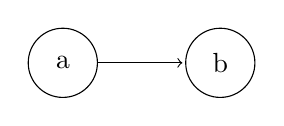
\begin{tikzpicture}[shorten >=1pt,node distance=2cm,on grid,auto] 
	\node[state] (a)   {a}; 
	\node[state] (b) [right=of a] {b}; 
	\path[->] 
	(a) edge  node {} (b)
	;
\end{tikzpicture}\\
The statement is incorrect. \\
Consider the graph G above, V = \{a, b\}, E = \{(a, b)\}.\\
The first DFS starting from a generates the following finishing time order: a, b.\\
In the second DFS, if the statement is true, b will be visited. \\
So the SCC of G is \{a, b\}, which is incorrect since obviously there are two SCCs in G: \{a\}, \{b\}\\

% 2
2.\\
Algorithm:\\
Run DFS. If there is a back edge, the graph contains a cycle. Otherwise, there is no cycle in the graph.\\

Correctness:\\
A directed graph G is acyclic if and only if a depth-first search of G yields no back edges(Lemma 22.11, ref[1]). So the algorithm is correct.\\

Time Complexity:\\
If there is no back edge, $|E| <= |V| + 1$, so the time complexity is $O(V)$ in stead of $O(|V|+|E|)$.\\
If there is a back edge, it will be found before visiting $|V|$ edges, so the time complexity is $O(V)$ in stead of $O(|V|+|E|)$.\\
Overall, the time complexity is $O(V)$.\\

Ref.\\
1. Cormen, T. (2013). Introduction to algorithms. 3rd ed. New Delhi: PHI Learning Private Ltd., p.614.\\

% 3
3.\\
\begin{algorithm}[H]
	\caption{DFS-MOD(G)}
	\For{each vertex u $\in$ G.V}
	{
		u.color = white\;
		u.$\pi$ = NIL\;
		cc[u] = 0\;
	}
	time = 0\;
	CCNum = 0\;
	\For{each vertex u $\in$ G.V}
	{
		\If{u.color == white}
		{
			DFS-VISIT-MOD(G, u, CCNum)\;
			CCNum ++\;
		}
	}
\end{algorithm}

\begin{algorithm}[H]
	\caption{DFS-VISIT-MOD(G, u, CCNum)}
	time = time + 1\;
	u.d = time\;
	u.color = GRAY\;
	cc[u] = CCNum\;
	\For{each v $\in$ G.Adj[u]}
	{
		\If{u.color == white}
		{
			v.$\pi$ = u\;
			DFS-VISIT-MOD(G, u, CCNum)\;
		}
	}
	u.color = BLACK\;
	time = time + 1\;
	u.f = time\;
\end{algorithm}

Explanation:\\
After modified DFS as stated above, the algorithm DFS-MOD will assign an integer label for each vertex. \\
If u, v are in the same connected component, u, v can be visited in the same DFS-VISIT-MOD iteration(Alg.1, line 10). So they will have the same integer(CCNum).\\
On the other hand, if u, v have the same integer(CCNum), they must be in the same DFS-VISIT-MOD iteration. So u can be visited from v using DFS, and v can be visited from u using DFS as well. So they are in the same connected component.\\

Ref.\\
1. Cormen, T. (2013). Introduction to algorithms. 3rd ed. New Delhi: PHI Learning Private Ltd., p.604.\\

% 4
4.\\
To prove $G^{SCC}=((G^T)^{SCC})^T$, we need to prove that they have the same vertex sets and edge sets.\\

step 1: Prove $V^{SCC} = ((V^T)^{SCC})^T$.\\
C is a SCC of G iff C is a SCC of $G^T$.\\
So $V^{SCC} = (V^T)^{SCC}$.\\
Since $(V^T)^{SCC} = ((V^T)^{SCC})^T$, $V^{SCC} = ((V^T)^{SCC})^T$.\\

step 2: Prove $E^{SCC} = ((E^T)^{SCC})^T$.\\
(1). Assume $(v_i, v_j) \in ((E^T)^{SCC})^T$.\\
So $(v_j, v_i) \in (E^T)^{SCC}$.\\
So $\exists x \in C_j, y \in C_i$ such that $(x, y) \in E^T$.\\
So $(y, x) \in E$, which means $\exists y \in C_i, x \in C_j$ such that $(y, x) \in E$.\\
Since $G$ and $G^T$ have the same SCC, $(v_i, v_j) \in E^{SCC}$.\\
So $E^{SCC} \supseteq ((E^T)^{SCC})^T$.\\
(2). Assume $(v_i, v_j) \in E^{SCC}$.\\
So $\exists x \in C_i, y \in C_j$ such that $(x, y) \in E$.\\
So $(y, x) \in E^T$, which means $\exists y \in C_j, x \in C_i$ such that $(y, x) \in E^T$.\\
Since $G$ and $G^T$ have the same SCC, $(v_j, v_i) \in (E^T)^{SCC}$.\\
So $(v_i, v_j) \in ((E^T)^{SCC})^T$.\\
So $E^{SCC} \subseteq ((E^T)^{SCC})^T$.\\
Based on (1) and (2), $E^{SCC} = ((E^T)^{SCC})^T$.\\

% 5
5a.\\
The statement is correct and can be proved by contradiction.\\
Assume there are two different MST A and B generated from G and $E^{diff}$ includes all the different edges in G.\\
Assume $e = (p, q) \in E^{diff}$ is the edge with the cheapest weight and, without loss of generality, assume $e \in A, e \notin B$.\\
So $B \bigcup \{e\}$ contains a cycle and at least one of these edges (named f) in the cycle has a larger weight.(Otherwise, since e is the edge with the cheapest weight in $E^{diff}$, all these edges are in the cycle are also in A, which form a cycle in A)
So $B \bigcup \{e\} \backslash {f}$ is also a MST and $w(B \bigcup \{e\} \backslash {f}) < w(B)$.\\
So B is not a MST. Contradiction.\\

5b.\\
The statement is incorrect.\\
Consider the following graph G:\\

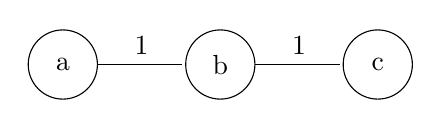
\begin{tikzpicture}[shorten >=1pt,node distance=2cm,on grid,auto] 
	\node[state] (a)   {a}; 
	\node[state] (b) [right=of a] {b}; 
	\node[state] (c) [right=of b] {c}; 
	\path[-] 
	(a) edge  node {1} (b)
	(b) edge  node {1} (c)
	;
\end{tikzpicture}\\

MST(G) is unique(MST(G) = G), but w((a, b)) = w((b, c)).\\

% 6
6.\\
Algorithm:\\
1. Use STRONGLY-CONNECTED-COMPONENTS algorithm (ref[1]) to find $G^{SCC}$.\\
2. Use TOPOLOGICAL-SORT algorithm (ref[2]) to find sorted vertex list of $G^{SCC}$(named nodeLis).\\
3. Go through the list and check whether there is an edge for each neighboring node pair nodeLis[i] and nodeLis[i + 1]. If all these edges exist, then for all pairs of vertices (u, v), either $u \rightsquigarrow v$ or $v \rightsquigarrow u$ or both holds. Otherwise, the conclusion doesn't hold.\\

Correctness:\\
If there is edges for each neighboring node pair in nodeLis.\\
For all the pairs of vertices $u, v \in V$, if u, v are in the same SCC, they will be connected.\\
If they are not in the same component, assume $u \in C_i, v \in C_j, i < j$. There is a path from $C_i$ to $C_j$ in nodeLis. So there is also a path from u to v.\\

Time Complexity:\\
1. SCC: $O(|V| + |E|)$\\
2. TOPOLOGICAL-SORT: $O(|V^{SCC}| + |E^{SCC}|) \leqslant O(|V| + |E|)$\\
3. Check edge: $O(|V^{SCC}|) \leqslant O(|V|)$\\
In total, the algorithm is linear-time.\\

Ref.\\
1. Cormen, T. (2013). Introduction to algorithms. 3rd ed. New Delhi: PHI Learning Private Ltd., p.617.\\
2. Cormen, T. (2013). Introduction to algorithms. 3rd ed. New Delhi: PHI Learning Private Ltd., p.613.\\

\end{document}
